\subsection{Hardware Tools}

\subsubsection{ESP32-S3 DevKit Microcontroller}

The ESP32-S3 DevKit is an economic and flexible MCU produced by Espressif Systems and used in numerous IoT devices and embedded platforms. It consists of two cores based on the 32-bit LX6 architecture of Xtensa processors, supports Wi-Fi and Bluetooth connectivity, and contains several peripheral components such as ADC, DAC, I2C, SPI, UART, PWM, and GPIO. These capabilities make the board useful for signal processing, controlling motors, and conducting reinforcement learning. Specifically, in the current project, the main task of the ESP32-S3 DevKit is handling RSSI collection and servo control for antenna alignment and performing reinforcement learning operations. The development environment of the firmware is Arduino IDE because it helps to prototype the system faster.

Since the ESP32-S3 DevKit board is installed in the main module, additional boards can be eliminated from the prototype design to have only one controller responsible for RSSI collection, actuator management, and debugging through the serial communication protocol.

\begin{figure}[H]
    \vspace{1em} 
    \centering
    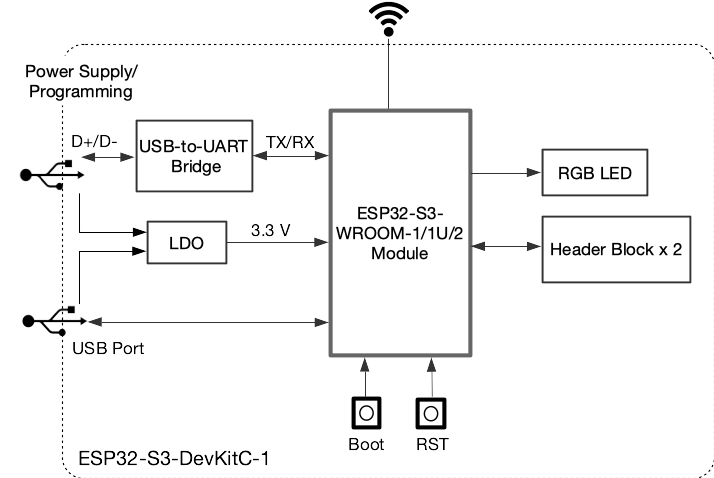
\includegraphics[width=0.8\textwidth]{images/esp32_block_diagram.png} 
    \vspace{0.2em}
    \caption[ESP32-S3 Block Diagram]{ESP32-S3 Block Diagram}
    \label{fig:esp32_block_diagram}
    \vspace{0.3em} 
    {\centering \small\itshape (Source: ESP32 Series Datasheet, Espressif Systems)\par}
\end{figure}

Figure~\ref{fig:esp32_block_diagram}  has the technical value as far as it shows the relevant parts of the physical board. The pins enable users to connect the hardware components necessary for PWM and motor control and supply power. The board also includes the buttons needed for programming and reconfiguration purposes. This figure proves the necessity of having an easy-to-manage programmable controller capable of communicating with other hardware elements of the module.

\vspace{0.5cm}
\begin{figure}[H]
    \centering
    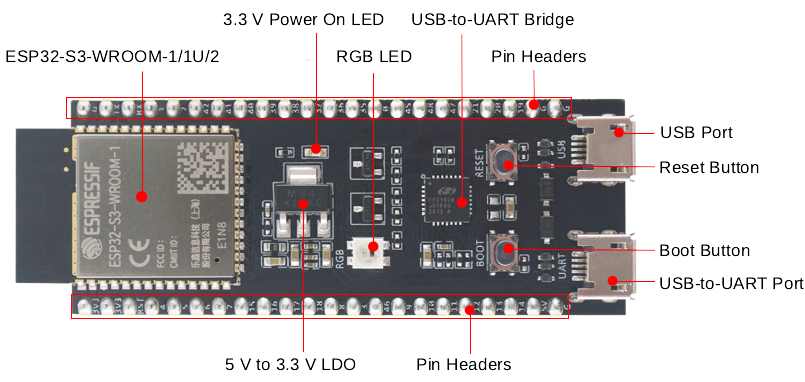
\includegraphics[width=0.8\textwidth]{images/esp32_gpio_diagram.png} 
    \vspace{0.2em}
    \caption[ESP32-S3 Components Description]{ESP32-S3 Components Description}
    \label{fig:esp32_gpio}
    \vspace{0.3em} 
    {\centering \small\itshape (Source: ESP32 Series Datasheet, Espressif Systems)\par}
\end{figure}

Figure~\ref{fig:esp32_gpio} is useful from an implementation perspective because it maps
the physical board elements that are directly relevant during prototyping. The exposed
pin headers provide the electrical interface for PWM, digital motor-control signals, and
power distribution, while the reset and boot buttons simplify firmware upload and test
iteration. This figure supports the practical requirement that the
controller must be easy to program, debug, and connect to the rest of the alignment
hardware.

\subsubsection{Stepper Motor}
Typically, the NEMA 17 stepper motor is associated with an angle of 1.8°, which implies that 200 steps occur per revolution. Microstepping, whereby the A4988 driver chip is used to increase the resolution, allows the reduction of full-step angles to 0.9°, 0.45°, or even finer increments, thereby providing the capability to precisely control antenna pointing towards optimal angles.

\begin{figure}[h]
    \vspace{1em}
    \centering
    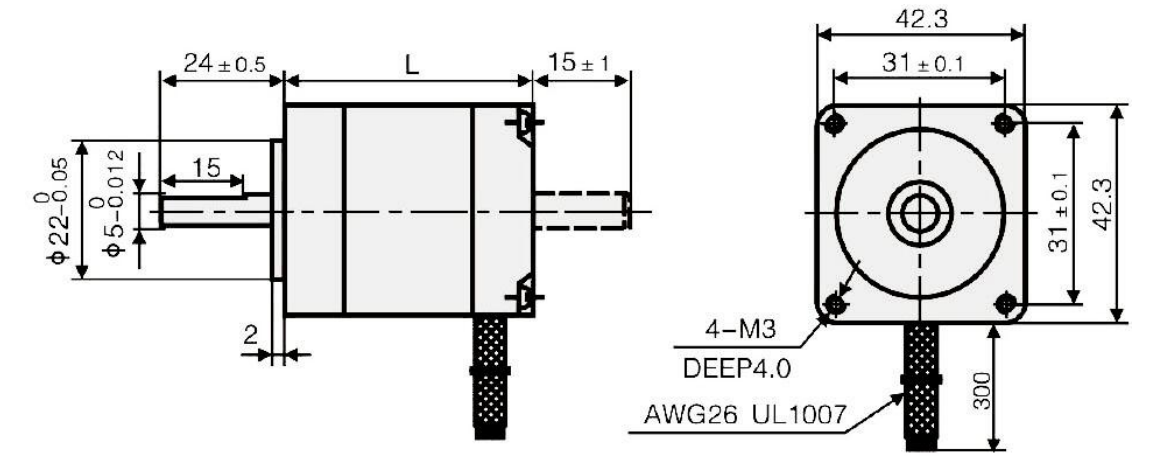
\includegraphics[width=1\textwidth]{images/motor.png} 
    \vspace{0.2em} 
    \caption[Nema 17 Stepper Motor Specification]{Nema 17 Stepper Motor Specification}
    \label{fig:stepper_motor}
    \vspace{0.3em} 
    {\centering \small\itshape (Source: ATO Nema 17 Stepper Motor Specs)\par}
\end{figure}

Figure~\ref{fig:stepper_motor} shows the physical specifications of the NEMA 17 motor, including its dimensions, as well as details on shaft and mounting hole dimensions. The physical parameters listed here can serve as guidelines for integration of the motor into the antenna mount design, including information on how to attach the motor to the turning platform and transmit azimuth torque effectively from the motor to the antenna mount.

A stepper motor can be connected directly to the ESP32 using a step/direction driver, such as the A4988. The step/direction combination allows one to control motor position with simple commands without having to use position sensors such as encoders. The selected motor operates in the voltage range of 12–24 V at currents of 1-2 A per phase. Stable operation of the motor is ensured by powering it with a DC source, thus avoiding voltage spikes that might interfere with accurate RSSI signal measurements. A stepper motor provides repeatable positioning without feedback since step motion is discrete; this is crucial for aligning anten


\subsubsection{Servo Motor}
For the control of the tilt angle of the antenna, the MG90S micro servo manufactured by TowerPro was adopted. It provides about 180° rotation range, and the resolution is ±1° per pulse. Therefore, it can provide precise tilt angle control when paired with the azimuth control driven by a stepper motor.

\begin{figure}[h]
    \vspace{1em}
    \centering
    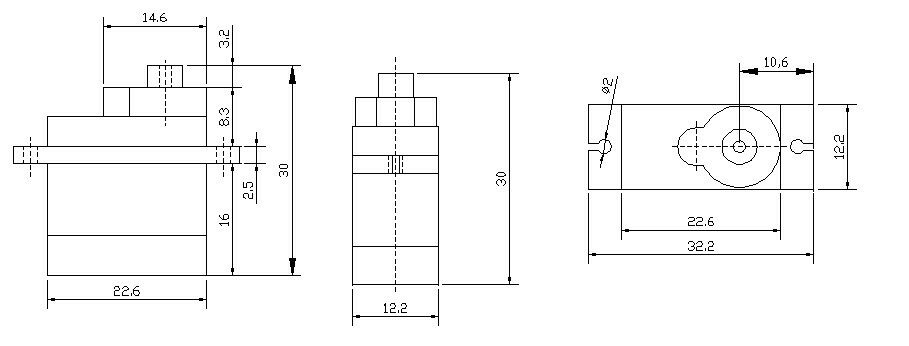
\includegraphics[width=1\textwidth]{images/mg90s_servo.png} 
    \vspace{0.2em} 
    \caption[TowerPro MG90S Micro Servo]{TowerPro MG90S Micro Servo}
    \label{fig:mg90s_servo}
    \vspace{0.3em} 
    {\centering \small\itshape (Source: TowerPro MG90S Datasheet)\par}
\end{figure}

The dimensions of the tilt actuator are shown in Figure~\ref{fig:mg90s_servo}. In this design, it is important that the tilt actuator should be compact since it is placed on the mobile part together with the antenna and controller components. The combination of a small footprint and the standard type of horn allows creating a lightweight tilt actuator that will not increase the moment of inertia of the rotating system.

MG90S works at an operating voltage of 4.8–6 VDC and has stall current consumption of up to 650 mA. Control is performed using conventional pulse width modulation pulses generated by the ESP32-S3 controller. In addition, a decoupling capacitor of 100 nF was installed on the power lines for filtering out the voltage spikes that may affect the microcontroller.

The MG90S servo provides precise positioning of the rotor angle, which is required for the antenna tilt angle control. It is lightweight, thereby minimizing the mechanical load of additional weight of the rotating parts, and its robust metal gears contribute to the longevity of the actuator.

\subsubsection{Motor Driver}
The A4988 is a complete microstepping driver designed for use with bipolar stepper motors; thus, enabling precise and easily executable control of the motor. It comes with five distinct step modes namely full, half, quarter, eighth, and sixteenth steps, with a maximum drive output capability of 35 V and 2 A, hence making it suitable for controlling NEMA 17 stepper motors within embedded applications. The A4988 makes it convenient to control the motor since it takes care of advancing the motor by one microstep per each STEP input pulse hence eliminating the necessity of complex phase sequencing and other control operations.

\begin{figure}[h]
    \vspace{1em}
    \centering
    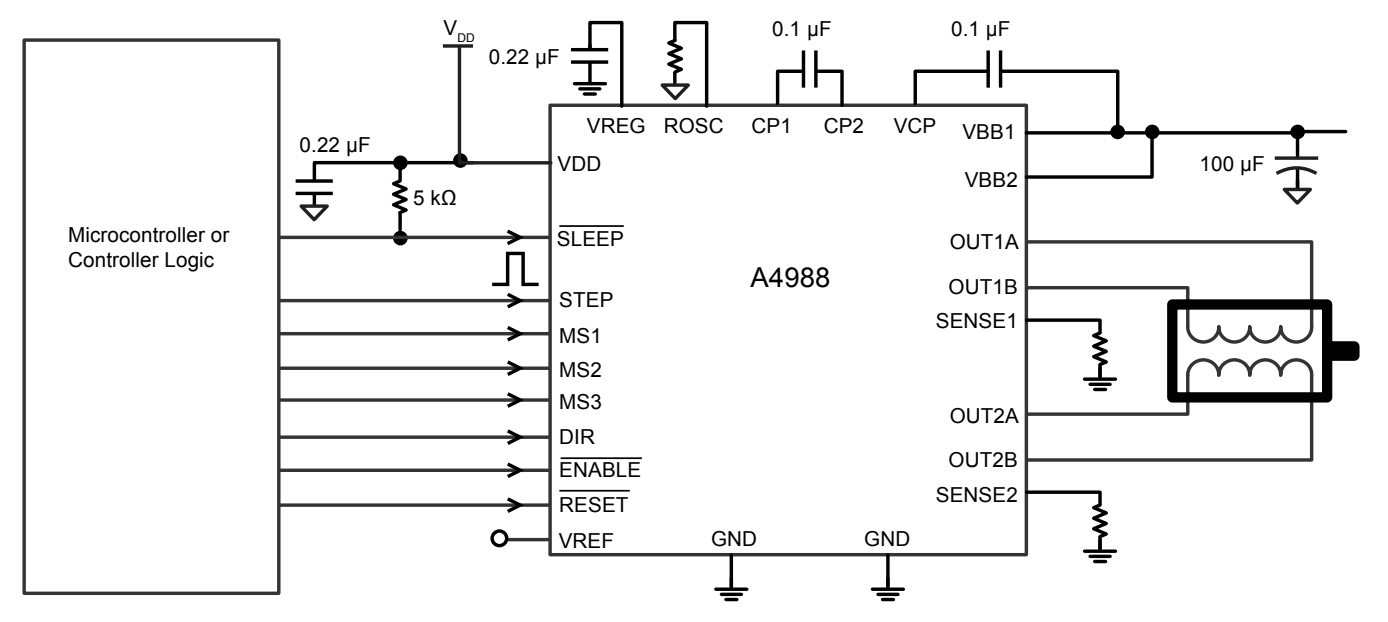
\includegraphics[width=1\textwidth]{images/motor_driver.png} 
    \vspace{0.2em} 
    \caption[A4988 Motor Driver Module Application Diagram]{A4988 Motor Driver Module Application Diagram}
    \label{fig:stepper_motor_driver}
    \vspace{0.3em} 
    {\centering \small\itshape (Source: Allegro Microsystems product documentation)\par}
\end{figure}

As seen from Figure~\ref{fig:stepper_motor_driver}, it can be noted that there is the relationship of signals being transferred from the microcontroller to the azimuth actuator. It is worth noting that the control signals used in this particular instance are relatively simple to handle by the microcontroller, which includes step input, direction input, and other signals related to step modes. In essence, the ESP32-S3 only needs to send control signals, while the A4988 takes care of handling the current-heavy phase drive of the motor.

The ESP32-S3 sends commands for step execution in relation to the alignment algorithm that is based on reinforcement learning, hence executing the exact number of steps required to align the directional antenna.

\subsubsection{Directional Antenna}
An antenna with a gain of 8-12 dBi and a frequency range of 2.35-2.55 GHz is selected in this design, specifically, a 2.4 GHz directional PCB panel Yagi antenna. Some of its features include:
\begin{itemize}
\item Main radiation lobe
\item Beam width of 30-60°
\item Variation of RSSI depending on orientation
\end{itemize}
All these specifications suit RSSI control and reinforcement learning applications because the signal gradient remains constant, and learning instability can be prevented. Moreover, its light weight ($\approx$19--40~g) ensures it can be fixed on small stepper motors without any additional mechanical resistance.

\begin{figure}[h]
    \vspace{1em}
    \centering
    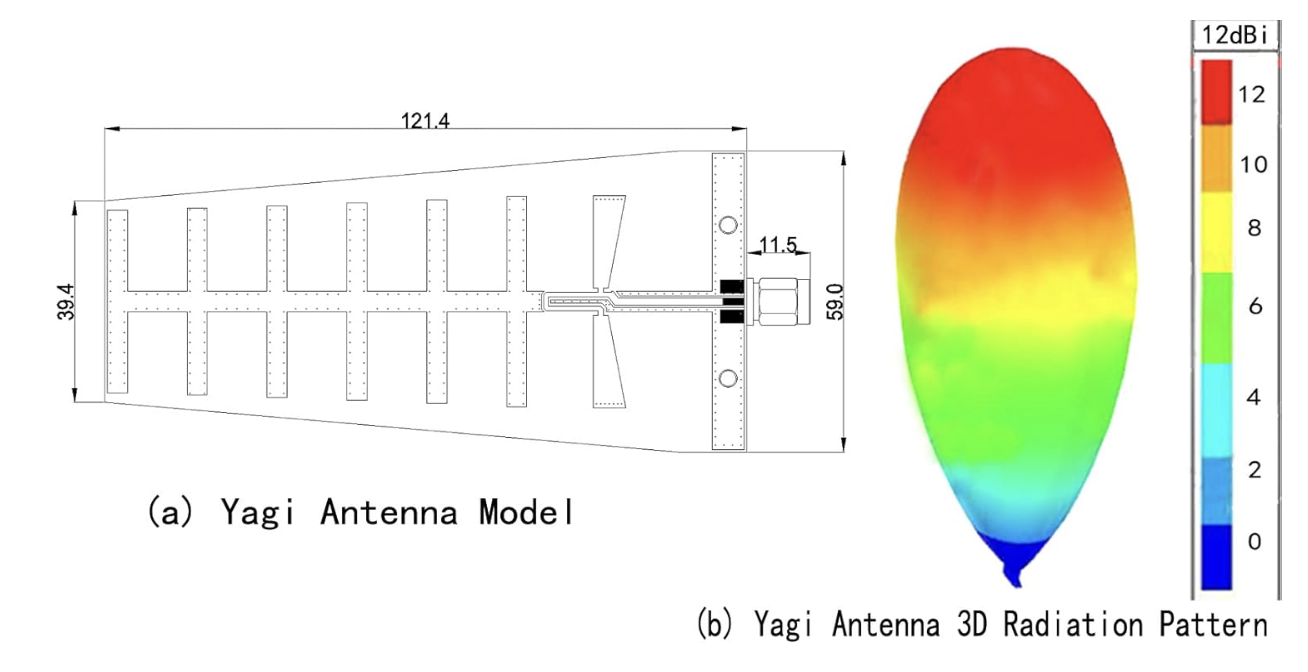
\includegraphics[width=1\textwidth]{images/antenna.png} 
    \vspace{0.2em} 
    \caption[High Gain 2.45GHz Directional Antenna]{High Gain 2.45GHz Directional Antenna}
    \label{fig:pcb_antenna}
    \vspace{0.3em} 
    {\centering \small\itshape (Source: Yagi Antenna Datasheet, ANTOSIYA)\par}
\end{figure}

Figure~\ref{fig:pcb_antenna} illustrates not only the antenna’s physical structure but also its radiation direction. The radiation lobe pattern verifies that there exists a main lobe; such characteristics become important in RSSI alignment since rotating the antenna leads to the signal strength modification. This characteristic guarantees that both controllers can identify good positions based on RSSI variations.

\subsubsection{RF Interfacing}

The directional antenna is connected to the receiving MCU using a short coaxial RF link to avoid any losses. The ESP32-S3 evaluation board has an u.FL (IPEX) RF connector that is connected to the antenna using an u.FL to SMA adapter cable. A short coaxial RF cable with SMA connectors is used between the adapter and the antenna element to ensure high signal quality while allowing rotational movements for the antenna assembly. All RF cables have an impedance of 50~$\Omega$, which is standard for 2.4 GHz wireless networks, thus reducing losses. Short and flexible coaxial cables also help reduce the mechanical load on the ESP32-S3 RF connector when the antenna is rotated.

\subsubsection{Power Supply and Management}

A reliable power delivery network is key for stable functioning of the designed antenna alignment algorithm in view of the concurrent presence of electromechanical actuators with high currents and RF and digital circuits sensitive to disturbances. For this reason, a dual rail power scheme is employed to isolate the domain of operation for logic supply voltages from the one for the motor drive voltage.

Namely, the ESP32-S3 microcontroller with its lower-power devices work on 5 V regulated, while the stepper motor receives higher voltage due to higher current and torque demands. Electrical isolation between the two domains prevents potential transfer of transients from the stepper motor power circuitry into the microcontroller and RF front end, thus helping prevent resets and data corruption in RSSI measurement circuitry.

{\setlength{\LTpre}{18pt}
 \setlength{\LTpost}{5pt}

\begin{longtable}{|
    >{\raggedright\arraybackslash}p{4.3cm} |
    >{\raggedright\arraybackslash}p{4.3cm} |
    >{\raggedright\arraybackslash}p{4.3cm} |}

\caption{Power Requirements of Major System Components}
\label{tab:power-management}\\
\hline
\textbf{Component} & \textbf{Operating Voltage} & \textbf{Typical Current} \\
\hline
\endfirsthead

\hline
\textbf{Component} & \textbf{Operating Voltage} & \textbf{Typical Current} \\
\hline
\endhead

ESP32-S3 Microcontroller & 5~V (regulated) & $\leq$ 500~mA \\
\hline
A4988 Motor Driver & 5~V & $\leq$ 50~mA \\
\hline
NEMA 17 Stepper Motor & 12~V & $\leq$ 1.2~A per phase \\
\hline
MG90S Servo Motor & 5~V (regulated) & $\leq$ 250~mA \\
\hline
\end{longtable}
}

In laboratory testing, a constant regulated power supply delivering 12 V and 3 A drives the stepper motor with the help of the A4988 IC. Another regulated supply delivering 5 V powers the ESP32 microcontroller with its periphery, either directly by an internal voltage regulator or externally. Mobile/untethered mode implies use of a 3S Lithium Polymer cell at 11.1 V nominal. The motor driver receives the 11.1V direct output from the battery pack, while the high-efficiency buck regulator converts the voltage to a stable 5 V supply for the ESP32 microcontroller. Decoupling capacitors are placed close to both regulators.